\section{Application-Specific Fault Tolerance}

\begin{frame}
  \frametitle{ULFM: User-Level Failure Mitigation}

  \centering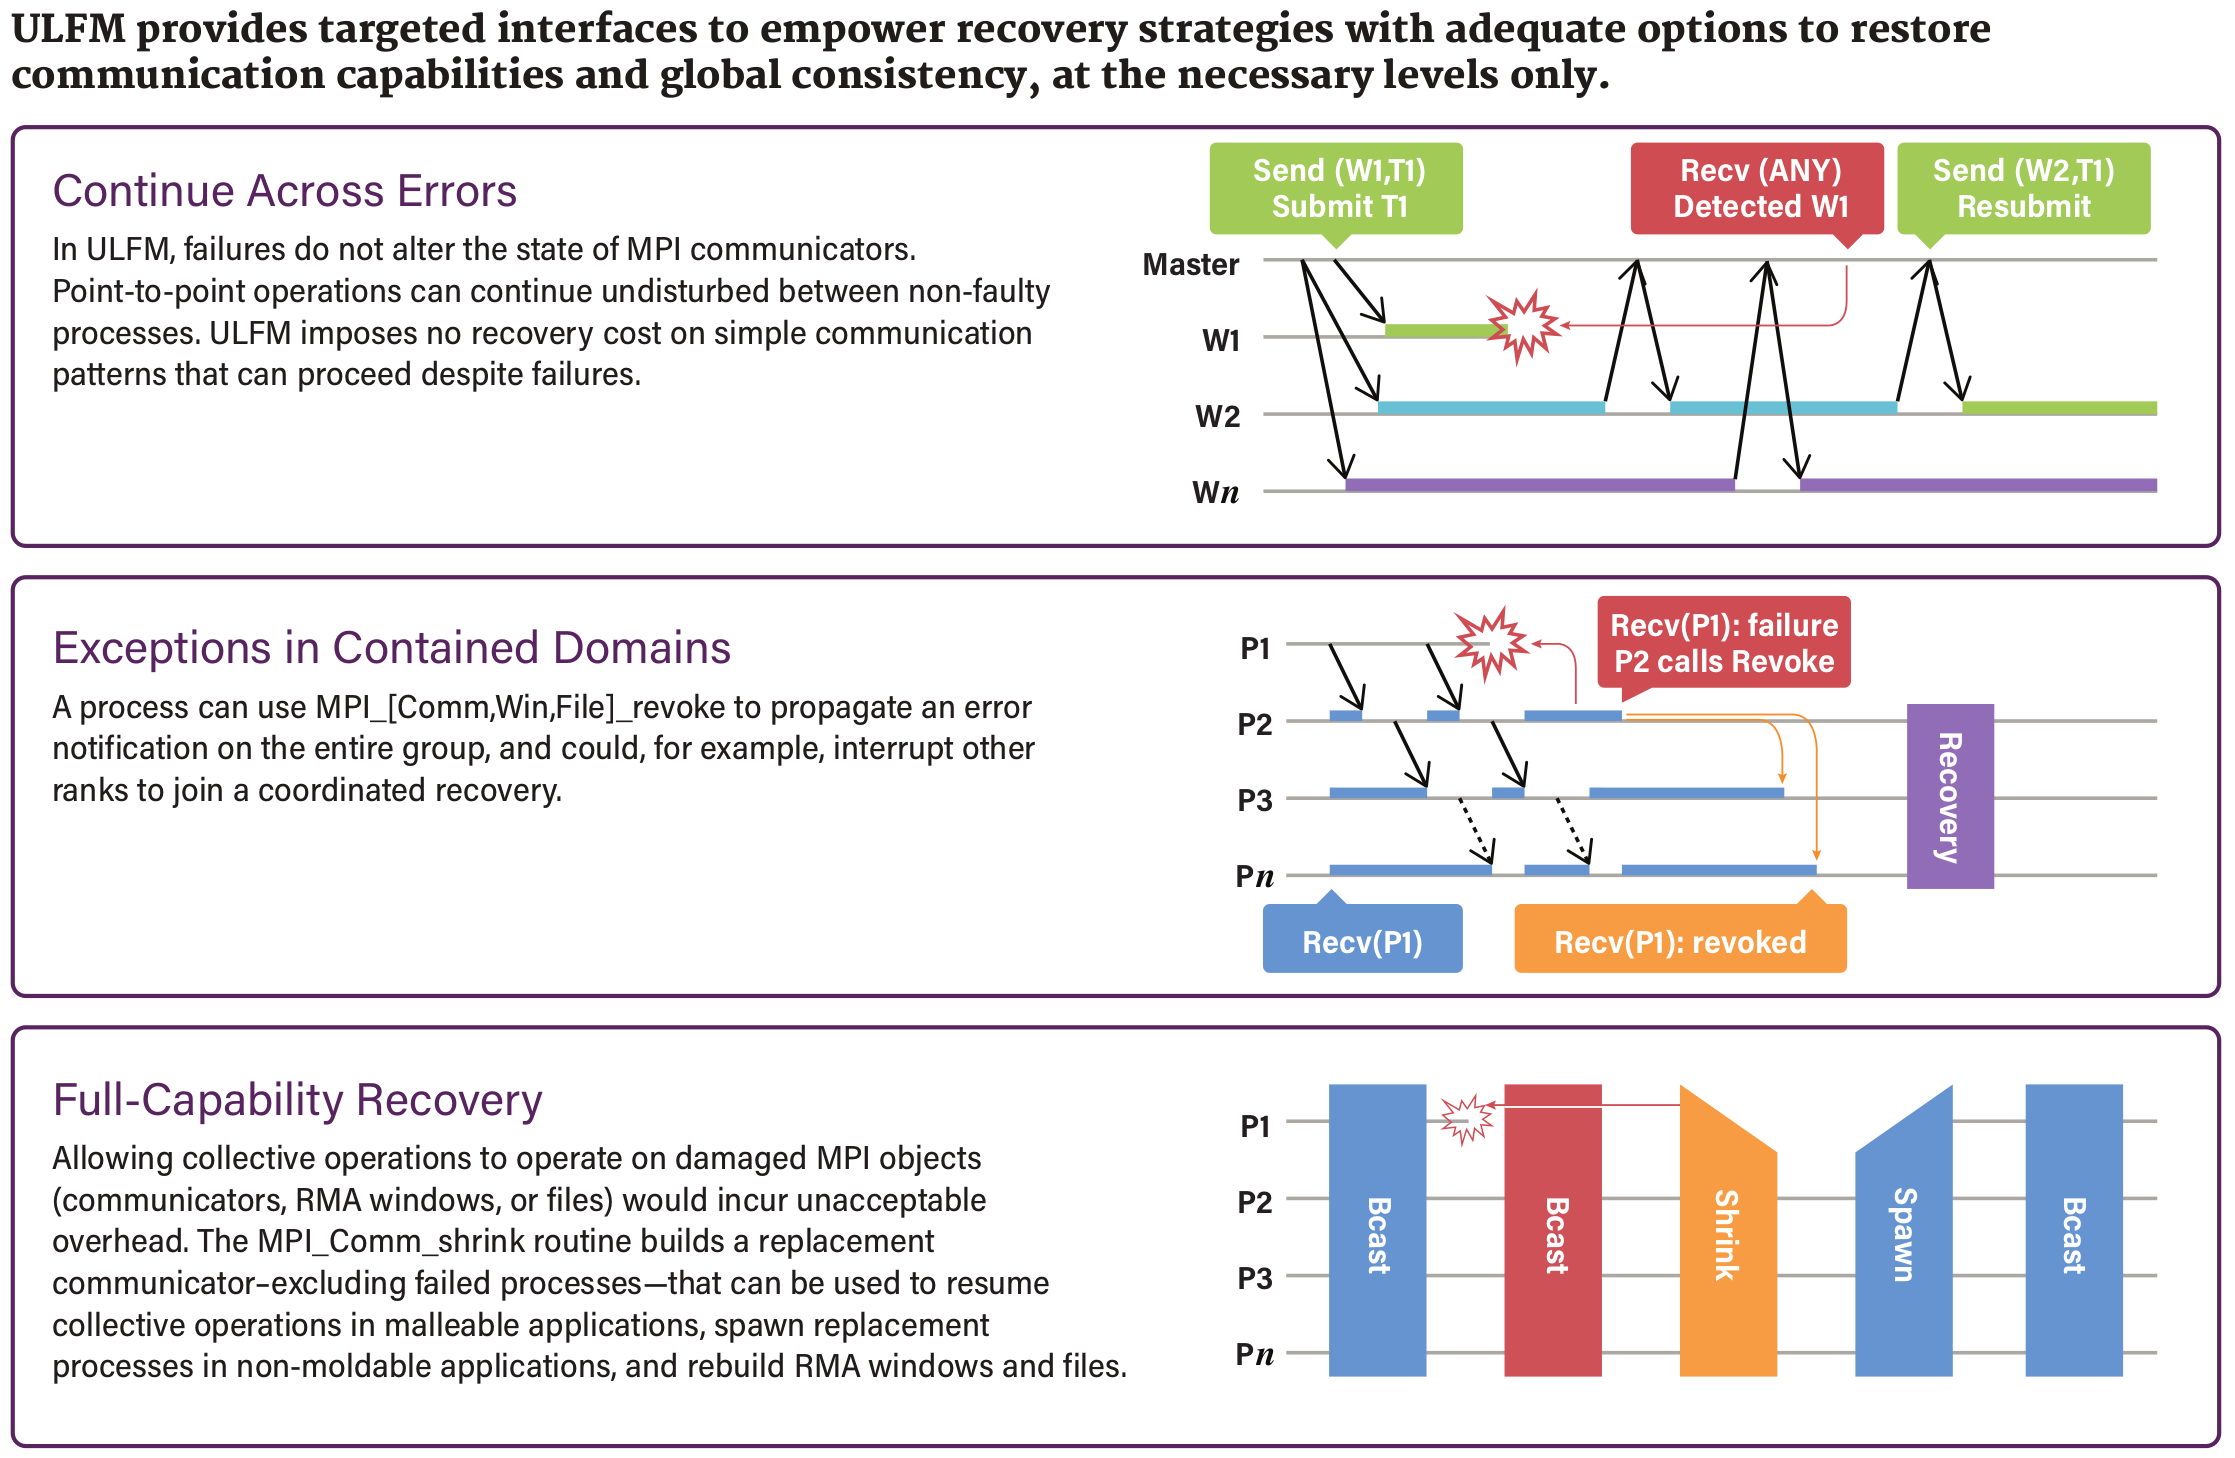
\includegraphics[height=.85\textheight]{ulfm.png}

\end{frame}


\newcommand{\processes}{\ensuremath{{\mathcal P}}}
\newcommand{\status}[2]{\ensuremath{S_{#1}^{#2}}}
\newcommand{\emitter}{\ensuremath{\texttt{emitter}}\xspace}
\newcommand{\observer}{\ensuremath{\texttt{observer}}\xspace}
\newcommand{\alive}{\ensuremath{\texttt{alive}}\xspace}
\newcommand{\dead}{\ensuremath{\texttt{dead}}}
\newcommand{\heartbeat}{\ensuremath{\textsc{heartbeat}}\xspace}
\newcommand{\timeoutping}{\ensuremath{\textsc{HB-Timeout}}\xspace}
\newcommand{\timeoutsuspect}{\ensuremath{\textsc{Susp-Timeout}}\xspace}
\newcommand{\timeout}[1]{\ensuremath{\textsc{Timeout}_{#1}}\xspace}
\newcommand{\newobserver}{\ensuremath{\textsc{NewObserver}}\xspace}
\newcommand{\findpred}{\ensuremath{\textit{FindEmitter}}\xspace}
\newcommand{\neighbors}{\ensuremath{\textit{Neighbors}}\xspace}
\newcommand{\broadcastmsg}{\ensuremath{\textsc{BcastMsg}}\xspace}
\newcommand{\pinginterval}{\ensuremath{\eta}\xspace}
\newcommand{\msgtime}{\ensuremath{\tau}\xspace}
\newcommand{\suspectinterval}{\ensuremath{\delta}\xspace}
\newcommand{\emittors}[1]{\ensuremath{M(#1)}}
\newcommand{\ringemittor}[1]{\ensuremath{M_R(#1)}}
\newcommand{\additionalemittors}[1]{\ensuremath{M_A(#1)}}
\newcommand{\receivers}[1]{\ensuremath{O(#1)}}
\newcommand{\ringreceiver}[1]{\ensuremath{O_R(#1)}}
\newcommand{\additionalreceivers}[1]{\ensuremath{O_A(#1)}}
\newcommand{\transfer}[2]{\ensuremath{T_{#1,#2}}}
\newcommand{\deadmsg}[1]{\ensuremath{\texttt{DeadMsg(\ensuremath{#1})}}}
\newcommand{\broadcastneighbors}[1]{\ensuremath{\mathcal B}_{#1}}
\newcommand{\deads}[1]{\ensuremath{{\mathcal D}_{#1}}}
\newcommand{\muind}{\ensuremath{\mu_{\text{ind}}}}
\newcommand{\ringalgorithm}{\textsc{RingAlgorithm}}

\newcommand{\probaSymbol}{\mathbb P}
\newcommand{\proba}[1]{\probaSymbol\left(#1\right)}

\tikzset{
  pics/lightning/.style 2 args={code={
      \draw [arrows={-stealth[scale=2]}] (#1) -- 
      ($(#1)!.5!(#2) + (.05,-.05)$) -- 
      ($(#1)!.5!(#2) + (-.05,.05)$) --
      (#2);
}}}

\usetikzlibrary{shadows,patterns,shapes}
\definecolor{bluetheme}{RGB}{0,128,255}

\tikzstyle{fancytitle} = [fill=bluetheme!40, text=black, rounded corners,inner sep=4pt] 
\tikzstyle{mybox} = [draw=bluetheme!40, fill=bluetheme!20, very thick, rectangle, rounded corners, inner ysep=10pt, drop shadow]

\tikzstyle{fancytitleR} = [fill=bluetheme, text=black, rounded corners,inner sep=4pt] 

\tikzstyle{myboxTitle} = [draw=bluetheme, fill=bluetheme, very thick, rectangle, rounded corners, inner ysep=10pt, drop shadow]

\tikzstyle{myboxR} = [draw=bluetheme, fill=bluetheme!20, very thick, rectangle, rounded corners, inner ysep=10pt]


\begin{frame}
  \frametitle{ULFM: Failure Detection and Notification}
  \begin{itemize}
  \item Default Failure Detection: TCP time-out ($\sim 20mn$)
  \item Default Failure Notification: Admin network
  \item Work on \textcolor{red}{fail-stop} errors assumes  \textcolor{red}{\emph{instantaneous}} failure detection
  \item Goals:
    \begin{itemize}
    \item Continue execution after crash of \textbf{several} nodes
    \item Need \emph{rapid} and \emph{global} knowledge of group members
      \begin{enumerate}
      \item \textcolor{red}{Rapid}: failure detection
      \item \textcolor{red}{Global}: failure notification
      \end{enumerate}
    \item Resilience mechanism should \textcolor{blue}{have minimal impact}
    \end{itemize}
  \end{itemize}
\end{frame}

\begin{frame}
\frametitle{Timeout techniques: $p$ observes $q$}
\begin{columns}
\begin{column}{0.75\textwidth}
\begin{itemize}
\item Pull technique
\begin{itemize}
\item Observer $p$ sends a \emph{Are you alive} message to $q$
\item[\textcolor{red}{\frownie}] More messages
\item[\textcolor{red}{\frownie}] Long timeout
\end{itemize}
\end{itemize}
\end{column}
\begin{column}{0.3\textwidth}
\centering
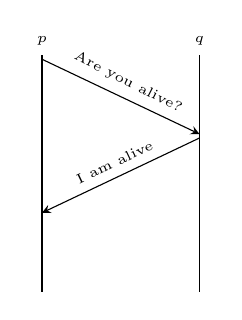
\begin{tikzpicture}
\draw (0, 3) -- (0, 0);
\node at (0,3) [font=\tiny,above]{$p$};
\draw (2, 3) -- (2, 0);
\node at (2,3) [font=\tiny,above]{$q$};
\draw [>=stealth,->] (0,2.95) -- (2,2) node [font=\tiny,midway,above,rotate=333] {Are you alive?};
\draw [>=stealth,->] (2,1.95) -- (0,1) node [font=\tiny,midway,above,rotate=25.40] {I am alive};
\end{tikzpicture}
\end{column}
\end{columns}

\begin{columns}
\begin{column}{0.75\textwidth}
\begin{itemize}
\item Push technique [1]
\begin{itemize}
\item Observed $q$ periodically sends heartbeats to $p$
\item[\textcolor{green}{\smiley}] Less messages
\item[\textcolor{green}{\smiley}] Faster detection (shorter timeout)
\end{itemize}
\end{itemize}
\end{column}
\begin{column}{0.3\textwidth}
\centering
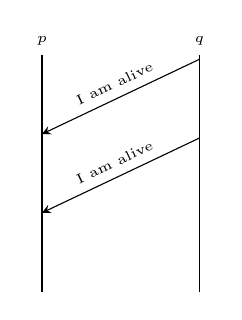
\begin{tikzpicture}
\draw (0, 3) -- (0, 0);
\node at (0,3) [font=\tiny,above]{$p$};
\draw (2, 3) -- (2, 0);
\node at (2,3) [font=\tiny,above]{$q$};
\draw [>=stealth,->] (2,2.95) -- (0,2) node [font=\tiny,midway,above,rotate=25.40] {I am alive};
\draw [>=stealth,->] (2,1.95) -- (0,1) node [font=\tiny,midway,above,rotate=25.40] {I am alive};
\end{tikzpicture}
\begin{tikzpicture}
\end{tikzpicture}
\end{column}
\end{columns}
\vfill
\scriptsize{[1]: W. Chen, S. Toueg, and M. K. Aguilera. On the quality of service of failure detectors. IEEE Trans. Computers, 2002}
\end{frame}

\begin{frame}
\frametitle{Algorithm for failure detection}

\begin{columns}
\begin{column}{0.5\textwidth}
\begin{itemize}
\item Processes arranged as a ring
\item Periodic heartbeats from a node to its successor
~\\
~\\
\item \textcolor{red}{Maintain ring of alive nodes}
\begin{itemize}
\item[$\rightarrow$] Reconnect ring after a failure
\item[$\rightarrow$] Inform all processes
\end{itemize}
\end{itemize}
\end{column}
\begin{column}{0.5\textwidth}
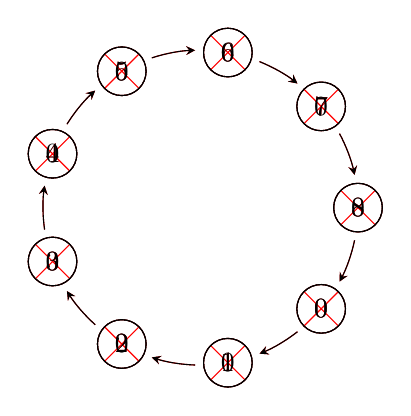
\begin{tikzpicture}[cross/.style={path picture={
  \draw[red]
(path picture bounding box.south east) -- (path picture bounding box.north west) (path picture bounding box.south west) -- (path picture bounding box.north east);
}}]
\def \n {9}
\def \radius {2cm}
\def \margin {12} 

\foreach \s in {1,...,\n}
{
  \pgfmathtruncatemacro\id{\n - \s}
  \ifthenelse{\s = 7 \OR \s = 6 \OR \s = 8 \OR \s = 2}
    {\node[draw, circle, red, cross] at ({360/\n * (\s - 1)}:\radius){$\id$};}
    {
        \ifthenelse{\s = 9}
                   {\node[draw, circle] at ({360/\n * (\s - 1)}:\radius){$0$};}
                   {\node[draw, circle] at ({360/\n * (\s - 1)}:\radius) {$\id$};};

    }
  \ifthenelse{\s = 6 \OR \s = 7}
  {\draw[->, >=stealth,red] ({360/\n * \s -\margin}:\radius)
    arc ({360/\n * \s - \margin}:{360/\n * (\s - 1)+\margin}:\radius);}
  {\draw[->, >=stealth] ({360/\n * \s - \margin}:\radius)
    arc ({360/\n * \s - \margin}:{360/\n * (\s - 1) + \margin}:\radius);}
}
\end{tikzpicture}
\end{column}
\end{columns}
\end{frame}




%\section{Failure propagation}



\begin{frame}
\frametitle{Reconnecting the ring}
\centering
\begin{overlayarea}{\textwidth}{\textwidth}
  {
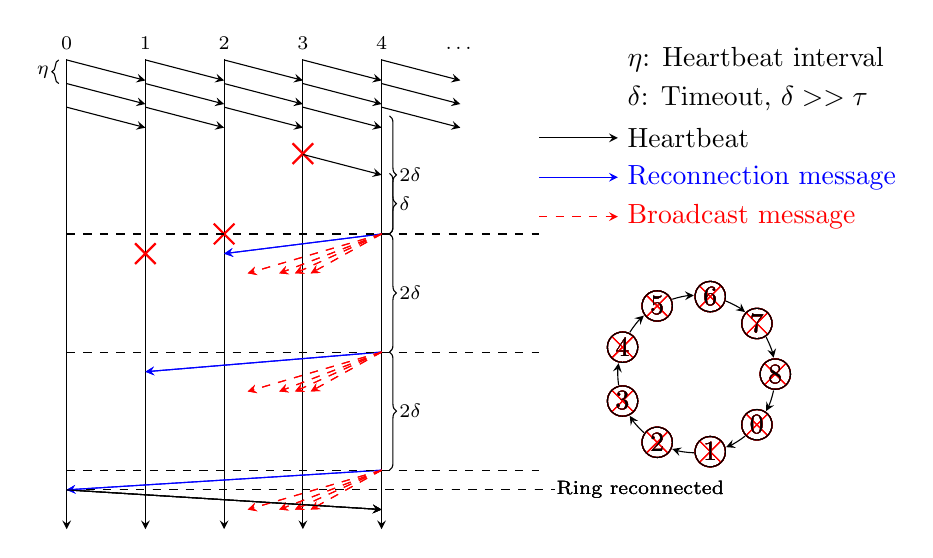
\begin{tikzpicture}[cross/.style={path picture={
  \draw[red]
(path picture bounding box.south east) -- (path picture bounding box.north west) (path picture bounding box.south west) -- (path picture bounding box.north east);
}}]
%%%%% position of the first process and distance between processes
%\begin{minipage}[t]{0.5\textwidth}
\def\z{0}
\def\s{1}
%%%%% lenght of the execution
\def\total{8}
%%%%% delta duration
\def\Tau{0.25}
\def\Eta{0.3}
\def\l{\total-4*\Eta}
\def\Delta{0.75}
%%%failure begin coordinate
\def\fb{0.01}
%%%failure end coordinate
\def\fe{0.50}
%%%% dashed lines for delta
\def\f{0.3}
%%%% number of faults
\def\nbf{3}
\def\propag{0.50}
\pgfmathsetmacro{\nbfmo}{\nbf - 1};
%%%%% beginning of reconnection tentative
\pgfmathsetmacro{\detect}{2 * \Delta}
\def\BeginRec{\l - \fb -\fb - \Tau - \Delta}
\def\Failure3{\BeginRec - \Tau - \Delta - \detect}
\def\EndRec{ \BeginRec - \nbfmo * \detect - \Tau - 2 * \Tau}
%\def\EndRec{\BeginBcast - \nbfmo * \propag - \propag}

%%failure free
  \draw [>=stealth,->] (\z - \s,\total) -- (\z - \s, \EndRec);
  \node at (\z - \s,\total) [font=\scriptsize,above]{$0$};

  \onslide<1-5>{\draw [>=stealth,->] (\z,\total) -- (\z, \EndRec);}
  \node at (\z,\total) [font=\scriptsize,above]{$1$};
\node [right] at (\z + 6, \total) {$\pinginterval$: Heartbeat interval};

\onslide<1-4>{\draw [>=stealth,->] (\z + \s,\total) -- (\z +\s, \EndRec);}
  \node at (\z + \s,\total) [font=\scriptsize,above]{$2$};

\draw [decoration={brace,mirror}, decorate] (\z - \s - 0.10,\total - \fb) -- (\z - \s - 0.10,\total - \fb - \Eta) node [black,midway, 
 left,font=\scriptsize,align=left]{$\pinginterval$};

\onslide<1>{\draw [>=stealth,->] (\z + 2*\s,\total) -- (\z + 2*\s, \EndRec);};
  \node at (\z + 2 * \s, \total) [font=\scriptsize,above]{$3$};

  \draw [>=stealth,->] (\z + 3*\s,\total) -- (\z + 3*\s, \EndRec);
  \node at (\z + 3*\s,\total) [font=\scriptsize,above]{$4$};
  \node at (\z + 4*\s,\total) [font=\scriptsize,above]{\ldots};
\draw [>=stealth,->] (\z + 5, \total - 1) -- (\z + 6, \total - 1) node [right]{Heartbeat};

\foreach \y in {0, 1, 2}
{
\foreach \x in {-1,0,1,2,3}
{  
  \draw  [>=stealth,->] (\z + \x * \s, \total - \fb - \y * \Eta) -- (\z+\x*\s+\s, \total - \fb - \fb - \Tau - \y * \Eta) node [font=\tiny,midway,rotate=331,below]{};
}
}

\onslide<2->{
%% failure of 3

  %  \draw (\z + 2*\s,\total) -- (\z + 2*\s, \l);
  \draw (\z + 2*\s,\total) -- (\z + 2*\s, \total-4*\Eta);
  \draw (\z + 2 * \s,\l) -- (\z + 2 * \s, \l) node [cross out, draw, red,
  thick]{};
  \onslide<3->{\draw [decoration={brace}, decorate] (\z + 3*\s + 0.10,\l - \Tau) -- (\z + 3*\s + 0.10,\BeginRec) node [black,midway, 
  right,font=\scriptsize,align=left]{$\suspectinterval$};}

  \onslide<5->{\draw (\z + \s,\total) -- (\z +\s, \BeginRec) node [cross out, draw, red,
  thick]{};}

\onslide<6->{
\draw (\z,\total) -- (\z,  \BeginRec - \Tau) node [cross out, draw, red,
  thick]{};;}

\draw  [>=stealth,->] (\z + 2*\s, \l - \fb) -- (\z+3*\s, \l - \fb - \fb - \Tau );

\foreach \x in {2,1,0}
{
  \pgfmathtruncatemacro{\y}{2 - \x};
  \pgfmathtruncatemacro{\i}{\x - 1};
  \pgfmathtruncatemacro{\anim}{\y + 3 + 1};

  \ifthenelse{\NOT \x = 0}
             {\onslide<\anim->{\draw [>=stealth,->,blue] (\z + 3 * \s, \BeginRec - \y * \detect) -- (\z + \i * \s, \BeginRec - \Tau - \y * \detect) node [font=\tiny,midway,rotate=15,below]{};
                 \onslide<7>{
                   \foreach \q in {1, 2, 3}
                      {
                        \draw [dashed,red,>=stealth,->] (\z + 3*\s,\BeginRec - \y * \detect) -- (\z + 1.5 *\s + 0.2*\q,\BeginRec - \y * \detect - \propag);
                      }
                      \draw [dashed,red,>=stealth,->] (\z + 3*\s,\BeginRec - \y * \detect) -- (\z + 1.3 *\s,\BeginRec - \y * \detect - \propag);
             }}}
             {\onslide<\anim->{\draw [>=stealth,->,blue] (\z + 3 * \s, \BeginRec - \y * \detect) -- (\z + \i * \s, \BeginRec - \Tau - \y * \detect) node [font=\tiny,midway,rotate=10,above]{};}}
             \pgfmathtruncatemacro{\anime}{\y + 4};
             \onslide<\anime->{\draw[dashed](\z -\s, \BeginRec - \y * \detect) -- (\z + 5*\s,  \BeginRec - \y * \detect);
               \ifthenelse{\y > 0}
                          {\draw [decoration={brace,mirror}, decorate] (\z + 3*\s + 0.10, \BeginRec - \y * \detect) -- (\z + 3*\s + 0.10, \BeginRec - \y * \detect + \detect) node [black,midway, 
                              right,font=\scriptsize,align=left]{2$\suspectinterval$};}{}
             }
             \onslide<\anim->{
               \onslide<7>{
                 \foreach \q in {1, 2, 3}
                    {
                      \draw [dashed,red,>=stealth,->] (\z + 3*\s,\BeginRec - \y * \detect) -- (\z + 1.5 *\s + 0.2*\q,\BeginRec - \y * \detect - \propag);
                    }
                    \draw [dashed,red,>=stealth,->] (\z + 3*\s,\BeginRec - \y * \detect) -- (\z + 1.3 *\s,\BeginRec - \y * \detect - \propag);
             }}
             \ifthenelse{\NOT \x = 0}{}
                        {\onslide<\anim->{
                            \draw [dashed] (-0.75, \BeginRec - \nbfmo * \detect - \Tau) -- (\z + 5 * \s + 0.20, \BeginRec - \nbfmo * \detect - \Tau);
                            \draw (\z + 5*\s + 0.10, \BeginRec - \nbfmo * \detect - \Tau) node [font=\scriptsize,right]{Ring reconnected}; 
%%%heartbeat of the healthy process
                            \draw  [>=stealth,->] (\z-\s, \BeginRec - \nbfmo * \detect - \Tau) -- (\z + 3*\s,  \BeginRec - \nbfmo * \detect - \Tau - \Tau) node [font=\tiny,midway,rotate=350,below]{};}
                        }
}

\onslide<3->{\node [right] at (\z + 6, \total-0.5) {$\suspectinterval$: Timeout, $\suspectinterval >> \msgtime$};}
%\node [left,font=\scriptsize] at (\z + 6, \total-2) {$\msgtime$: Message transmission upper bound};}
\onslide<4->{\draw [>=stealth,->,blue ](\z + 5, \total-1.5) -- (\z + 6, \total-1.5) node [right]{Reconnection message};}
\onslide<7->{\draw [>=stealth,->,dashed,red ](\z + 5, \total-2) -- (\z + 6, \total-2) node [right]{Broadcast message};}

%%% T(3)
%% \draw [dashed] (-0.75, \l - \fb - \fb) -- (3, \l - \fb - \fb);
%% \draw [dashed] (-0.75, \EndRec) -- (3, \EndRec);
%% \draw [>=stealth,<->] (-0.75, \l - \fb - \fb) -- (-0.75, \EndRec) node [font=\scriptsize,left,midway]{$T(\nbf,C)$};

%% \draw (3.25, \EndRec - 0.10) rectangle (6.25,\EndRec - 0.65 - 0.10 - 0.20);
%% \draw node at (3.25, \EndRec - 0.10 - 0.15) [font=\scriptsize,right]{HB=\heartbeat};
%% \draw node at (3.25, \EndRec - 0.10 - 0.40) [font=\scriptsize,right,blue]{NO=\newobserver};
%% \draw node at (3.25, \EndRec - 0.10 - 0.65) [font=\scriptsize,right,red]{Bcast=Broadcast Operation};
}

\def \n {9}
\def \radius {1}
\def \margin {12}
%\node[circle, red, cross,right of=fin] at ({360/\n * 2 - 110}:\radius){7};
%\node[circle, red, cross,right of=fin] at ($(fin.south west)+(3,0)$){6};
\draw node at (\z + 5*\s,  \BeginRec - \detect)(fin){};
%\node(A)[draw,circle,right of=fin,xshift=1cm,yshift=1cm]{0};

\foreach \s in {1,...,\n}
{
  \pgfmathtruncatemacro\id{\n - \s}
  \onslide<1>{
    \node[draw, circle,right of=fin,xshift=6cm,yshift=4cm,inner sep=1pt] at ({360/\n * (\s - 1)}:\radius) {$\id$};
  }
  \onslide<2-4>{
    \ifthenelse{\id = 3}
       {\node[draw,circle, red, cross,right of=fin,xshift=6cm,yshift=4cm,circle,inner sep=1pt] at ({360/\n * (\s - 1)}:\radius){$\id$};}
       {
         \node[draw, circle,right of=fin,xshift=6cm,yshift=4cm,inner sep=1pt] at ({360/\n * (\s - 1)}:\radius) {$\id$};
       }
  }
  \onslide<5>{
    \ifthenelse{\id = 3 \OR \id=2}
             {\node[draw,circle, red, cross,right of=fin,xshift=6cm,yshift=4cm,circle,inner sep=1pt] at ({360/\n * (\s - 1)}:\radius){$\id$};}
             {
               \node[draw, circle,right of=fin,xshift=6cm,yshift=4cm,inner sep=1pt] at ({360/\n * (\s - 1)}:\radius) {$\id$};
             }
  }
  \onslide<6->{
    \ifthenelse{\id = 3 \OR \id=2 \OR \id=1}
               {\node[draw,circle,red,cross,right of=fin,xshift=6cm,yshift=4cm,circle,inner sep=1pt] at ({360/\n * (\s - 1)}:\radius){$\id$};}
               {
                 \node[draw, circle,right of=fin,xshift=6cm,yshift=4cm,inner sep=1pt] at ({360/\n * (\s - 1)}:\radius) {$\id$};
               }
  }
%% \ifthenelse{\s = 6 \OR \s = 7}
  %% {\draw[->, >=stealth,red] ({360/\n * \s -\margin}:\radius)
  %%   arc ({360/\n * \s - \margin}:{360/\n * (\s - 1)+\margin}:\radius);}%|- (\z+5,\total-2)
  \draw[->, >=stealth,xshift=7cm,yshift=4cm] ({360/\n * \s - \margin}:\radius)
    arc ({360/\n * \s - \margin}:{360/\n * (\s - 1) + \margin}:\radius);
}

\end{tikzpicture}
}
\end{overlayarea}
\end{frame}

\begin{frame}
  \frametitle{Failure Notification}

  \begin{columns}
    \begin{column}{0.6\textwidth}
      \begin{itemize}
      \item Hypercube Broadcast Algorithm
        \begin{itemize}
        \item Recursive doubling broadcast algorithm by each node
        \item Completes if $f \leq \lfloor log(n)\rfloor - 1$ ($f$: number of failures, $n$: number of alive processes)
        \item Completes within $2 \tau log(n)$
        \end{itemize}
        \vfill
      \item Application to failure detector
        \begin{itemize}
        \item If $n \neq 2^l$
          \begin{itemize}
          \item $k = \lfloor log(n) \rfloor$ 
          \item $2^k \leq  n  \leq 2^{k+1}$
          \item Initiate two successive broadcast operations
          \end{itemize}
        \item Source $s$ of broadcast sends its current list $D$ of dead processes
        \item {\scriptsize No update of $D$ during broadcast initiated by $s$ -- (do NOT change broadcast topology on the fly)}
        \end{itemize}
      \end{itemize}
    \end{column}

    \begin{column}{0.4\textwidth}
      \centering
      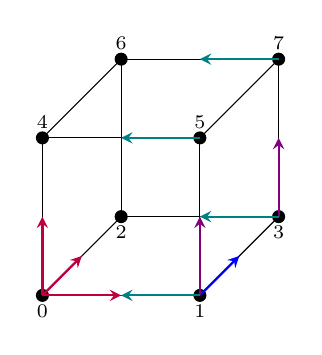
\begin{tikzpicture}
        \def\size{2}
        \def\decalage{1}
        \def\arrowLength{1}
        \foreach \x in {0, 1}
                 {
                   \draw (\x*\decalage,\size+\x*\decalage) -- (\size+\x*\decalage,\size+\x*\decalage);
                   \node [circle,fill=black,scale=0.5] at (\x*\decalage,\size+\x*\decalage){};
                   \pgfmathtruncatemacro{\id}{\x*\decalage*2+4};
                   \node [above,font=\scriptsize] at  (\x*\decalage,\size+\x*\decalage){\id};%{\pgfmathparse{\x*\decalage*2+4}\pgfmathresult};
                   \draw (\x*\decalage,\x*\decalage) -- (\x*\decalage,\size+\x*\decalage);
                   \node [circle,fill=black,scale=0.5] at (\x*\decalage,\x*\decalage){};
                   \pgfmathtruncatemacro{\id}{\x*\decalage*2};
                   \node [below,font=\scriptsize] at (\x*\decalage,\x*\decalage){\id};
                   \draw (\size+\x*\decalage,\size+\x*\decalage) -- (\size+\x*\decalage,\x*\decalage);
                   \node [circle,fill=black,scale=0.5] at (\size+\x*\decalage,\size+\x*\decalage){};
                   \pgfmathtruncatemacro{\id}{\x*\decalage*2+5};
                   \node [above,font=\scriptsize] at (\size+\x*\decalage,\size+\x*\decalage){\id};
                   \draw (\x*\decalage,\x*\decalage) -- (\size+\x*\decalage,\x*\decalage);
                   \node [circle,fill=black,scale=0.5] at (\size+\x*\decalage,\x*\decalage){};
                   \pgfmathtruncatemacro{\id}{\x*\decalage*2+1};
                   \node [below,font=\scriptsize] at (\size+\x*\decalage,\x*\decalage){\id};
                 }
        \draw(0, \size) -- (\decalage, \size+\decalage);
        \draw(\size, \size) -- (\decalage+\size, \size+\decalage);
        \draw(0, 0) -- (\decalage, \decalage);
        \draw(\size, 0) -- (\size+\decalage, \decalage);
        \draw [>=stealth,->,purple,thick] (0,0) -- (\arrowLength,0);
        \draw [>=stealth,->,purple,thick] (0,0) -- (0,\arrowLength);
        \draw [>=stealth,->,purple,thick] (0,0) -- (\arrowLength/2,\arrowLength/2);
        \draw [>=stealth,->,blue,thick] (\size,0) -- (\arrowLength/2+\size,\arrowLength/2);
        \draw [>=stealth,->,violet,thick] (\size,0) -- (\size,\arrowLength);
        \draw [>=stealth,->,violet,thick] (\size+\decalage,\decalage) -- (\size+\decalage,\decalage+\arrowLength);
        \draw [>=stealth,->,teal,thick] (\size,0) -- (\arrowLength,0);
        \draw [>=stealth,->,teal,thick] (\size+\decalage,\decalage) -- (\arrowLength+\decalage,\decalage);
        \draw [>=stealth,->,teal,thick] (\size,\size) -- (\size-\arrowLength,\size);
        \draw [>=stealth,->,teal,thick] (\size+\decalage,\size+\decalage) -- (\size-\arrowLength+\decalage,\size+\decalage);
      \end{tikzpicture}

      \scriptsize
      \begin{tabular}{|c|c|c|c|}
        \hline
        Node & Node1 & Node2 & Node4\\\hline
        1 & \onslide<1->0 & \onslide<1->{0-2-3} &  \onslide<1->{0-4-5}\\
        2 & \onslide<1->{0-1-3} & \onslide<1->0 & \onslide<1->{0-4-6}\\
        3 & \onslide<1->{0-1} & \onslide<1->{0-2} & \onslide<1->{0-4-5-7}\\
        4 & \onslide<1->{0-1-5} & \onslide<1->{0-2-6} & \onslide<1-> 0\\
        5 & \onslide<1->{0-1} & \onslide<1->{0-2-6-7} & \onslide<1->{0-4}\\
        6 & \onslide<1->{0-1-3-7} & \onslide<1->{0-2} & \onslide<1->{0-4}\\
        7 & \onslide<1->{0-1-3} & \onslide<1->{0-2-6} & \onslide<1->{0-4-5}\\\hline
        \end{tabular}
    \end{column}
  \end{columns}

\end{frame}

\begin{frame}
\frametitle{Worst-case analysis}
\begin{center}
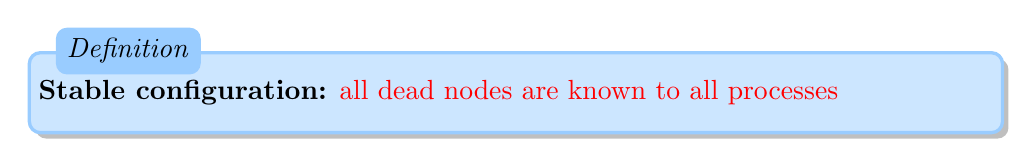
\begin{tikzpicture}
\node [mybox] (box) { %
  \begin{minipage}{1.0\textwidth}
\textbf{Stable configuration:}  \textcolor{red}{all dead nodes are known to all processes}
  \end{minipage}
};
\node [fancytitle, right=10pt] at (box.north west) {\text{\emph{Definition}}};
\end{tikzpicture}
  
\begin{tikzpicture}
\draw [>=stealth,|->](0,5) -- (10,5) node [font=\tiny,below left]{Time}; 
\draw (3,5.10) -- (3,4.90);
\node at (1.50,4.90)[below,font=\scriptsize]{Stable};
\draw (8,5.10) -- (8,4.90);
\node at (9,4.90)[below,font=\scriptsize]{Stable};
\node at (5.5,4.90)[below,font=\scriptsize]{at most $T(f)$ if $f$ faults};
\pic [red] {lightning={3.20,5.5}{3,5}};
%\draw [>=stealth, ->] (3.5, 5.5) -- (3, 5) ;
\pic [red] {lightning={3.70,5.5}{3.5,5}};
\pic [red] {lightning={4.20,5.5}{4,5}};
\node at (3.5,5.5) [above,font=\tiny]{Failures};
\pic [red] {lightning={5.20,5.5}{5,5}};
\pic [red] {lightning={5.70,5.5}{5.5,5}};
\pic [red] {lightning={7.2,5.5}{7,5}};

%\draw [>=stealth,->](0,5) -- (5,10) node [font=\tiny,below left]{Time}; 
\end{tikzpicture}
\end{center}

\begin{theorem}
With $n \leq N$ alive nodes, and for any $f \leq \lfloor \log n \rfloor -1$,
we have
\begin{equation*}
T(f) \leq  f(f+1)  \suspectinterval + f \msgtime + \frac{f(f+1)}{2}(8 \msgtime \log n)
\end{equation*}
\end{theorem}
\begin{itemize}
\item 2 sequential broadcasts: $4 \tau log n$
\item One-port model: broadcast messages and heartbeats interleaved
\end{itemize}

\end{frame}

\begin{frame}
\frametitle{Worst-case scenario}

$$\begin{array}{cccc}
T(f) \leq  & \underbrace{f(f+1)  \suspectinterval  +   f \msgtime}  & + &  \underbrace{\frac{f(f+1)}{2}(8 \msgtime \log n)}\\
& \textcolor{red}{reconstruction} & & \textcolor{blue}{broadcast}
\end{array}$$

\begin{itemize}
\item $T(f) \leq  \text{ring reconstruction} + \text{broadcasts}$ (for the proof)
\item \textcolor{blue}{Process $p$ discovers the death of $q$ at most \textbf{once}\\
$\Rightarrow$ $i-th$ dead process discovered dead by at most $f-i+1$ processes\\
$\Rightarrow$ at most $\frac{f(f+1)}{2}$ broadcasts}
\item \textcolor{red}{$R(f)$ ring reconstruction time\\
For $ 1 \leq f \leq \lfloor \log n \rfloor -1$,
$$R(f) \leq  R(f-1) + 2f  \suspectinterval + \msgtime$$}
\end{itemize}
\end{frame}

\begin{frame}
\frametitle{Ring reconnection}

\begin{columns}
\begin{column}{0.5\textwidth}

$$R(f) \leq  R(f-1) + 2f  \suspectinterval + \msgtime$$

\begin{itemize}
\item $R(1) \leq 2 \msgtime + \suspectinterval  \leq 2  \suspectinterval + \msgtime$
\item $R(f) \leq R(f-1) + R(1)$\\
if next failure \emph{non-adjacent}
to previous ones
\item Worst-case when failing nodes consecutive in the ring
\item Build the ring by  \emph{``jumping''} over platform
to avoid correlated failures
\end{itemize}
\end{column}
\begin{column}{0.5\textwidth}
\scalebox{0.7}{%
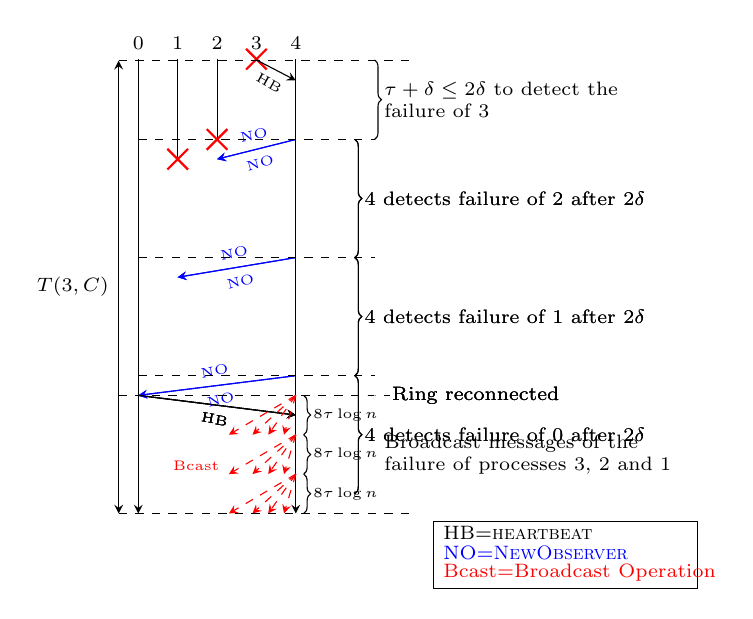
\begin{tikzpicture}
%%%%% position of the first process and distance between processes
%\begin{minipage}[t]{0.5\textwidth}
\def\z{0}
\def\s{0.5}
%%%%% lenght of the execution
\def\l{6}
%%%%% delta duration
\def\Tau{0.25}
\def\Delta{0.75}
%%%failure begin coordinate
\def\fb{0.01}
%%%failure end coordinate
\def\fe{0.50}
%%%% dashed lines for delta
\def\f{0.3}
%%%% number of faults
\def\nbf{3}
\def\propag{0.50}
\pgfmathsetmacro{\nbfmo}{\nbf - 1};
%%%%% beginning of reconnection tentative
\pgfmathsetmacro{\detect}{2 * \Delta}
\def\BeginRec{\l - \fb -\fb - \Tau - \Delta}
\def\Failure3{\BeginRec - \Tau - \Delta - \detect}
\def\BeginBcast{ \BeginRec - \nbfmo * \detect - \Tau}
\def\EndRec{\BeginBcast - \nbfmo * \propag - \propag}
%\foreach \x \in {1, 2, 4}
%{

%}
%%   \draw [>=stealth,->] (\z + 4*\s,\l) -- (\z + 4*\s, \EndRec);
%%   \node at (\z + 4 * \s,\l) [font=\scriptsize,above]{$5$};

  \draw [>=stealth,->] (\z - \s,\l) -- (\z - \s, \EndRec);
  \node at (\z - \s,\l) [font=\scriptsize,above]{$0$};

  \draw [>=stealth,->] (\z + 3*\s,\l) -- (\z + 3*\s, \EndRec);
  \node at (\z + 3*\s,\l) [font=\scriptsize,above]{$4$};
%%% nodes
  \draw (\z + 2 *\s,\l) -- (\z + 2 * \s, \l) node [cross out, draw, red,
  thick]{};
%  \node at (\z,\l) [font=\scriptsize,above]{$1$};
%\draw (\z + \s,\l) -- (\z + \s, \BeginRec - \Tau - \detect - \Tau - \fb )node [cross out, draw, red,
  \draw (\z + \s,\l) -- (\z +\s, \BeginRec) node [cross out, draw, red,
  thick]{};
\node at (\z + \s,\l) [font=\scriptsize,above]{$2$};
\draw (\z,\l) -- (\z,  \BeginRec - \Tau) node [cross out, draw, red,
  thick]{};;
\node at (\z,\l) [font=\scriptsize,above]{$1$};

%\draw (\z, \l) -- (\z, \l - \fb - \fb) node [cross out, draw, red,
%  thick]{};
\node at (\z + 2 * \s, \l) [font=\scriptsize,above]{$3$};


%%%% heartbeat
\draw  [>=stealth,->] (\z + 2*\s, \l - \fb) -- (\z+3*\s, \l - \fb - \fb - \Tau ) node [font=\tiny,midway,rotate=331,below]{HB};
%%% explanation for failure detection
\draw [decoration={brace}, decorate] (\z + 4*\s + 0.5,\l - \fb) -- (\z + 4*\s + 0.5,\BeginRec) node [black,midway,
  right,font=\scriptsize,align=left]{$\msgtime + \suspectinterval \leq 2 \suspectinterval$ to detect the \\ failure of $3$};


%%%%% Failures detection of 2 delimitation
%\draw[dashed](\z -\s, \BeginRec - \Tau - \Delta) -- (\z + 5*\s,  \BeginRec - \Tau - \Delta);
%\draw [decoration={brace}, decorate] (\z + 4*\s + 0.25, \BeginRec) -- (\z + 4*\s + 0.25,\BeginRec - \Tau - \Delta) node [black,midway,
%  right,font=\tiny,align=left]{$3$ detects failure of $2$ after $R(1)$\\ This failure increases the size \\ of the segment $I_1=\{1\}$ by one};



%%%% 4 detects 3's failure
%\draw [decoration={brace}, decorate] (\z + 4*\s + 0.25, \Failure3) -- (\z + 4*\s + 0.25,\Failure3 - \Tau - \Delta) node [black,midway,
%  right,font=\tiny,align=left]{$4$ detects failure of $3$ after $R(1)$\\ This failure increases the size of \\ the segment $I_1=\{1,2\}$ by one};


%%%% 4's reconnection messages
\foreach \x in {2,1,0}
{
  \pgfmathtruncatemacro{\y}{2 - \x};
  \pgfmathtruncatemacro{\i}{\x - 1};
  \ifthenelse{\NOT \x = 0}
             {\draw [>=stealth,->,blue] (\z + 3 * \s, \BeginRec - \y * \detect) -- (\z + \i * \s, \BeginRec - \Tau - \y * \detect) node [font=\tiny,midway,rotate=15,below]{NO};}
             {\draw [>=stealth,->,blue] (\z + 3 * \s, \BeginRec - \y * \detect) -- (\z + \i * \s, \BeginRec - \Tau - \y * \detect) node [font=\tiny,midway,rotate=10,above]{NO};}
  \draw[dashed](\z -\s, \BeginRec - \y * \detect) -- (\z + 5*\s,  \BeginRec - \y * \detect);
\ifthenelse{\NOT \x = 0}{
\ifthenelse{\x = 2}{
  \draw [decoration={brace}, decorate] (\z + 4*\s + 0.25, \BeginRec - \y * \detect) -- (\z + 4*\s + 0.25,\BeginRec - \y * \detect - \detect) node [black,midway,
 right,font=\scriptsize,align=left]{$4$ detects failure of $\x$ after $2\suspectinterval$};}
{
  \draw [decoration={brace}, decorate] (\z + 4*\s + 0.25, \BeginRec - \y * \detect) -- (\z + 4*\s + 0.25,\BeginRec - \y * \detect - \detect) node [black,midway,
 right,font=\scriptsize,align=left]{$4$ detects failure of $\x$ after $2\suspectinterval$};}
}
{
\draw [dashed] (-0.75, \BeginRec - \nbfmo * \detect - \Tau) -- (\z + 5 * \s + 0.20, \BeginRec - \nbfmo * \detect - \Tau);
\draw (\z + 5*\s + 0.10, \BeginRec - \nbfmo * \detect - \Tau) node [font=\scriptsize,right]{Ring reconnected};
%%%heartbeat of the healthy process
\draw  [>=stealth,->] (\z-\s, \BeginRec - \nbfmo * \detect - \Tau) -- (\z + 3*\s,  \BeginRec - \nbfmo * \detect - \Tau - \Tau) node [font=\tiny,midway,rotate=350,below]{HB};
}
}


%%%% Broadcast begin
\foreach \x in {1,...,\nbf}
{
  \pgfmathtruncatemacro{\y}{\x - 1};
  \pgfmathtruncatemacro{\p}{4 - \x};
\foreach \q in {1, 2, 3}
{
  \draw [dashed,red,>=stealth,->] (\z + 3*\s,\BeginBcast - \y * \propag) -- (\z + 1.5 *\s + 0.2*\q,\BeginBcast - \y * \propag - \propag);
}

%\ifthenelse{\x = 2}
%{  \draw [dashed,red,>=stealth,->] (\z + 3*\s,\BeginBcast - \y * \propag) -- (\z + 1.3 *\s,\BeginBcast - \y * \propag - \propag);
 \draw [dashed,red,>=stealth,->] (\z + 3*\s,\BeginBcast - \y * \propag) -- (\z + 1.3 *\s,\BeginBcast - \y * \propag - \propag);
  \draw [decoration={brace}, decorate] (\z + 3 *\s + 0.10,\BeginBcast - \y * \propag) -- (\z + 3*\s + 0.10,\BeginBcast - \propag - \y * \propag) node [black,midway,
  right,font=\tiny,align=left]{$8 \msgtime \log n$};
}

\draw node at (\z + 1.3 *\s,\BeginBcast -  \propag - \propag  + 0.10) [font=\tiny,left,red]{Bcast};

\draw [decoration={brace}, decorate,white] (\z + 3 *\s + 1,\BeginBcast) -- (\z + 3*\s + 1,\BeginBcast -  \nbf * \propag) node [black,midway,
  right,font=\scriptsize,align=left]{Broadcast messages of the \\ failure of processes $3$, $2$ and $1$};

%%% T(3)
\draw [dashed] (-0.75, \l - \fb - \fb) -- (3, \l - \fb - \fb);
\draw [dashed] (-0.75, \EndRec) -- (3, \EndRec);
\draw [>=stealth,<->] (-0.75, \l - \fb - \fb) -- (-0.75, \EndRec) node [font=\scriptsize,left,midway]{$T(\nbf,C)$};

\draw (3.25, \EndRec - 0.10) rectangle (6.60,\EndRec - 0.65 - 0.10 - 0.20);
\draw node at (3.25, \EndRec - 0.10 - 0.15) [font=\scriptsize,right]{HB=\heartbeat};
\draw node at (3.25, \EndRec - 0.10 - 0.40) [font=\scriptsize,right,blue]{NO=\newobserver};
\draw node at (3.25, \EndRec - 0.10 - 0.65) [font=\scriptsize,right,red]{Bcast=Broadcast Operation};

%\draw[dashed](0, \l - \fb) -- (5, \l - \fb);

%% \foreach \x in {1,3}
%% {
%%   \pgfmathtruncatemacro{\y}{3 - \x};
%%   \draw[dashed](\z -\s, \BeginRec - \y * \detect - \y * \Tau) -- (\z + 5*\s,  \BeginRec - \y * \detect - \y * \Tau);
%% }
%% \draw[dashed](\z -\s, \BeginRec - 3 * \detect - 2 * \Tau) -- (\z + 5*\s,  \BeginRec - 3 * \detect - 2 * \Tau);

\end{tikzpicture}
}
\end{column}
\end{columns}
\end{frame}

\begin{frame}
\frametitle{Noise}
\hspace*{-0.5cm}
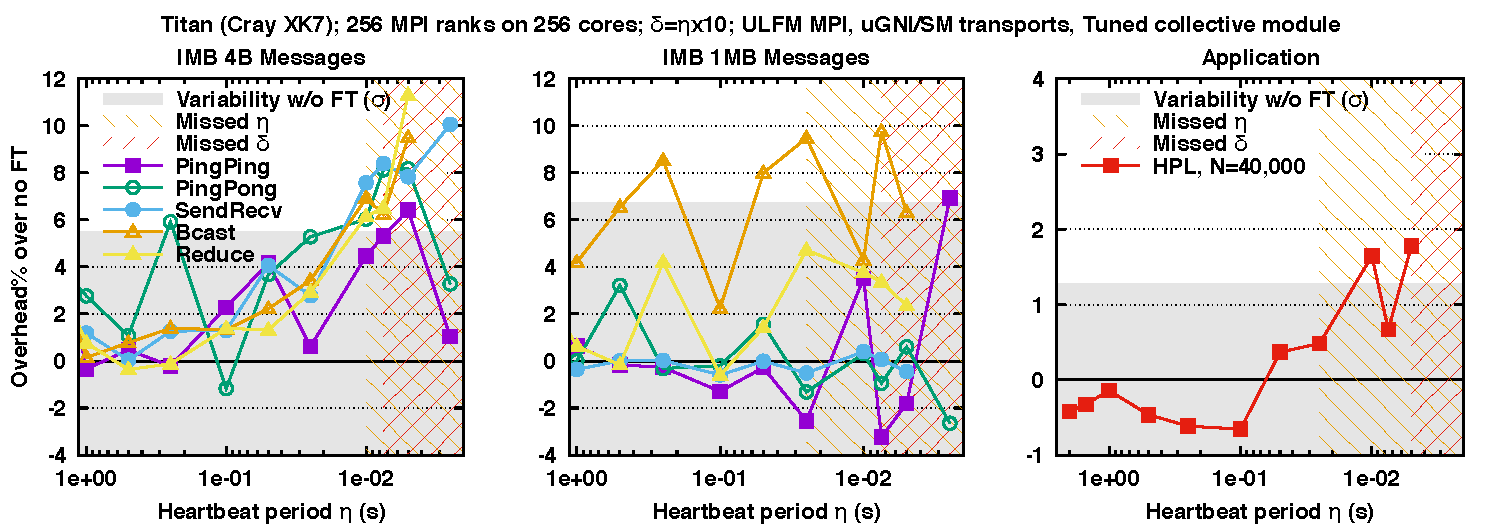
\includegraphics[width=1.1\textwidth]{etanoise-titan.pdf}
\end{frame}

\begin{frame}
\frametitle{Detection and propagation delay}
\hspace*{-0.5cm}
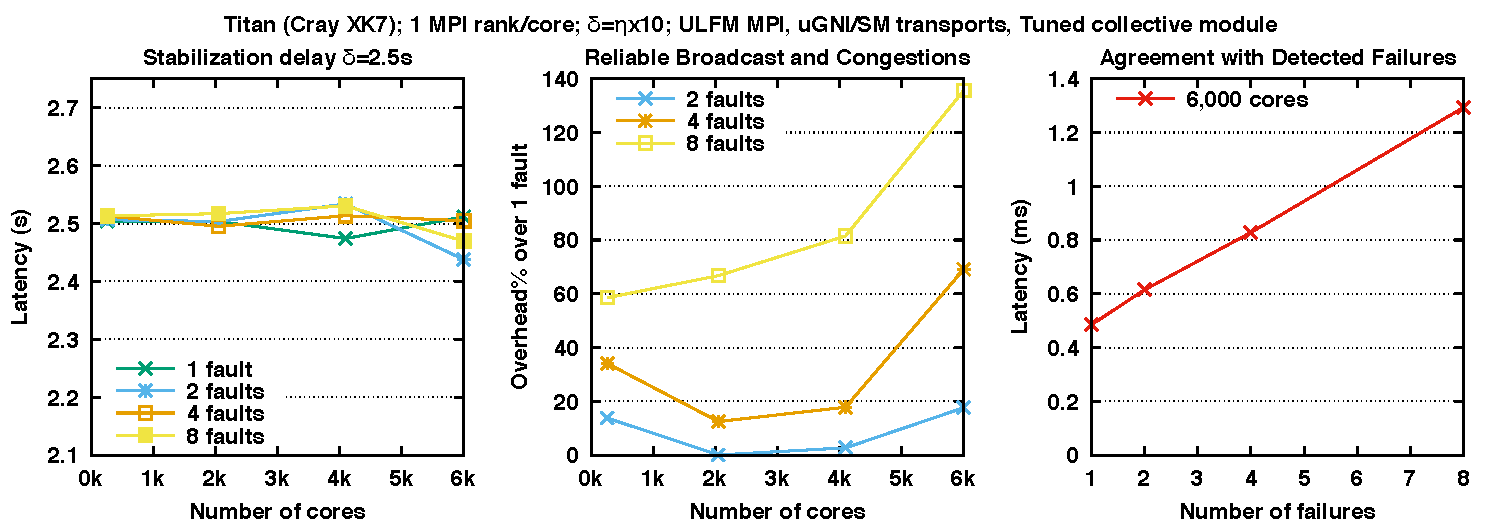
\includegraphics[width=1.1\textwidth]{recva-titan.pdf}
\end{frame}

\begin{frame}
  \frametitle{Algorithm-Based Fault Tolerant LU over ULFM}

  \begin{columns}
    \begin{column}{.3\textwidth}
      \begin{itemize}
      \item Algorithm-Based Fault Tolerant LU (PDGETRF) based on ULFM
        \begin{itemize}
        \item Replication to ensure checksum availability
        \item Partial checkpoint to rollback Q-panel operation
        \item ABFT to recover most of the missing data
        \item Partial re-execution to recover panel
        \end{itemize}
      \end{itemize}
    \end{column}
    \begin{column}{.7\textwidth}
        \begin{center}
          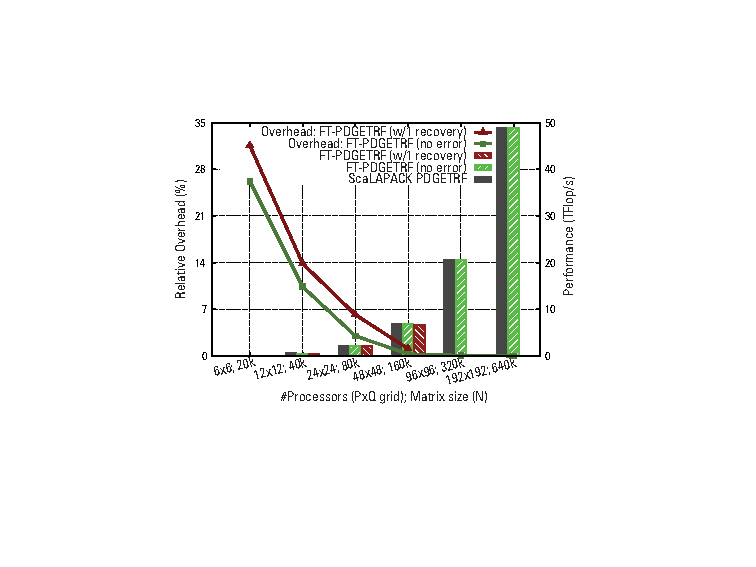
\includegraphics[width=.9\linewidth]{abftlu-perf.pdf}
        \end{center}
    \end{column}
  \end{columns}
\end{frame}

\begin{frame}
  \frametitle{Conclusion on Application-Specific Fault Tolerance}

  \begin{itemize}
  \item Many applications are amenable to 'Roll-Forward' approaches
    \begin{itemize}
    \item No Re-Execution, no TLost! (or very little)
    \end{itemize}
  \item Performance of roll-forward is orders of magnitude higher than checkpoint/restart
    \begin{itemize}
    \item And it scales better!
    \end{itemize}
  \item Roll-forward is only for specific parts of real life applications
    \begin{itemize}
    \item But we have composition techniques! (see manuscript)
    \end{itemize}
  \item Roll-forward requires a resilient communication middleware
    \begin{itemize}
    \item ULFM is integrated in Open MPI and MPICH
    \item Overhead on failure-free is non measurable
    \item Overhead on failure-specific operation is very small
    \item It is slowly being integrated in the MPI Standard
    \end{itemize}
  \end{itemize}
  
\end{frame}
